\subsection{Socioeconomic Status}
Socioeconomic status can play a crucial role in terms of the ability to afford healthcare, access to doctors \& medication, healthy food etc. Interestingly, in figure \ref{fig:socioecoau} we can see that through the years the most disadvantaged mothers had babies. To have a deeper insight we looked into state-based data. We can see (figure\ref{fig:socioecostates}) different trends in different states. We can observe that in some states such as ACT, NSW \& NT more advantaged the mothers are more interested they are in having babies. Interestingly, we can see the opposite trend in QLD, SA \& Tasmania where often the least advantaged mothers tend to have more babies.

\begin{figure}
  \centering
  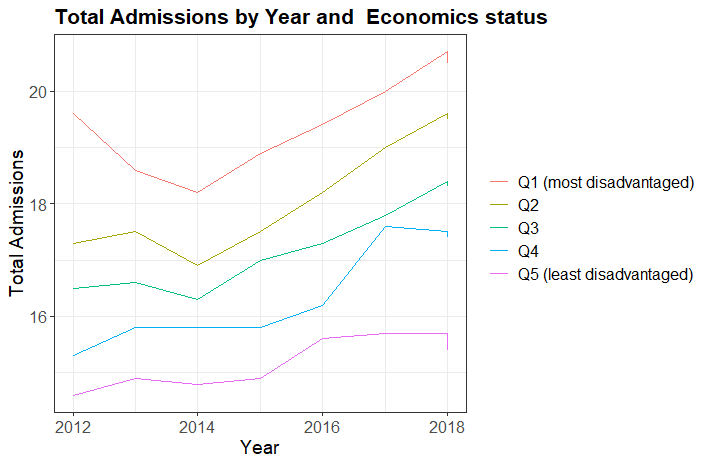
\includegraphics[width=1\textwidth]{subsections/socioeco/economic_status_au.png}
  \caption{Socioeconomic status of mothers in Australia.}
  \label{fig:socioecoau}
\end{figure}

\begin{figure}
  \centering
  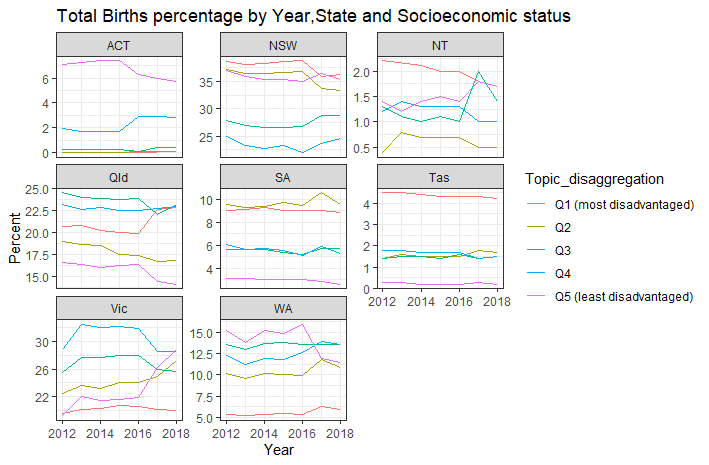
\includegraphics[width=1\textwidth]{subsections/socioeco/socio_economic.png}
  \caption{Socioeconomic status of mothers in different states.}
  \label{fig:socioecostates}
\end{figure}